% Options for packages loaded elsewhere
\PassOptionsToPackage{unicode}{hyperref}
\PassOptionsToPackage{hyphens}{url}
%
\documentclass[
  ignorenonframetext,
  aspectratio=32,
]{beamer}
\usepackage{pgfpages}
\setbeamertemplate{caption}[numbered]
\setbeamertemplate{caption label separator}{: }
\setbeamercolor{caption name}{fg=normal text.fg}
\beamertemplatenavigationsymbolshorizontal
% Prevent slide breaks in the middle of a paragraph
\widowpenalties 1 10000
\raggedbottom
\setbeamertemplate{part page}{
  \centering
  \begin{beamercolorbox}[sep=16pt,center]{part title}
    \usebeamerfont{part title}\insertpart\par
  \end{beamercolorbox}
}
\setbeamertemplate{section page}{
  \centering
  \begin{beamercolorbox}[sep=12pt,center]{section title}
    \usebeamerfont{section title}\insertsection\par
  \end{beamercolorbox}
}
\setbeamertemplate{subsection page}{
  \centering
  \begin{beamercolorbox}[sep=8pt,center]{subsection title}
    \usebeamerfont{subsection title}\insertsubsection\par
  \end{beamercolorbox}
}
\AtBeginPart{
  \frame{\partpage}
}
\AtBeginSection{
  \ifbibliography
  \else
    \frame{\sectionpage}
  \fi
}
\AtBeginSubsection{
  \frame{\subsectionpage}
}

\usepackage{amsmath,amssymb}
\usepackage{iftex}
\ifPDFTeX
  \usepackage[T1]{fontenc}
  \usepackage[utf8]{inputenc}
  \usepackage{textcomp} % provide euro and other symbols
\else % if luatex or xetex
  \usepackage{unicode-math}
  \defaultfontfeatures{Scale=MatchLowercase}
  \defaultfontfeatures[\rmfamily]{Ligatures=TeX,Scale=1}
\fi
\usepackage{lmodern}
\usetheme[]{AnnArbor}
\usecolortheme{lily}
\ifPDFTeX\else  
    % xetex/luatex font selection
\fi
% Use upquote if available, for straight quotes in verbatim environments
\IfFileExists{upquote.sty}{\usepackage{upquote}}{}
\IfFileExists{microtype.sty}{% use microtype if available
  \usepackage[]{microtype}
  \UseMicrotypeSet[protrusion]{basicmath} % disable protrusion for tt fonts
}{}
\makeatletter
\@ifundefined{KOMAClassName}{% if non-KOMA class
  \IfFileExists{parskip.sty}{%
    \usepackage{parskip}
  }{% else
    \setlength{\parindent}{0pt}
    \setlength{\parskip}{6pt plus 2pt minus 1pt}}
}{% if KOMA class
  \KOMAoptions{parskip=half}}
\makeatother
\usepackage{xcolor}
\newif\ifbibliography
\setlength{\emergencystretch}{3em} % prevent overfull lines
\setcounter{secnumdepth}{-\maxdimen} % remove section numbering


\providecommand{\tightlist}{%
  \setlength{\itemsep}{0pt}\setlength{\parskip}{0pt}}\usepackage{longtable,booktabs,array}
\usepackage{calc} % for calculating minipage widths
\usepackage{caption}
% Make caption package work with longtable
\makeatletter
\def\fnum@table{\tablename~\thetable}
\makeatother
\usepackage{graphicx}
\makeatletter
\newsavebox\pandoc@box
\newcommand*\pandocbounded[1]{% scales image to fit in text height/width
  \sbox\pandoc@box{#1}%
  \Gscale@div\@tempa{\textheight}{\dimexpr\ht\pandoc@box+\dp\pandoc@box\relax}%
  \Gscale@div\@tempb{\linewidth}{\wd\pandoc@box}%
  \ifdim\@tempb\p@<\@tempa\p@\let\@tempa\@tempb\fi% select the smaller of both
  \ifdim\@tempa\p@<\p@\scalebox{\@tempa}{\usebox\pandoc@box}%
  \else\usebox{\pandoc@box}%
  \fi%
}
% Set default figure placement to htbp
\def\fps@figure{htbp}
\makeatother

\makeatletter
\@ifpackageloaded{float}{}{\usepackage{float}}
\floatstyle{plain}
\@ifundefined{c@chapter}{\newfloat{algo}{h}{loalgo}}{\newfloat{algo}{h}{loalgo}[chapter]}
\floatname{algo}{Algorithm}
\newcommand*\listofalgos{\listof{algo}{List of Algorithms}}
\makeatother
\makeatletter
\@ifpackageloaded{caption}{}{\usepackage{caption}}
\AtBeginDocument{%
\ifdefined\contentsname
  \renewcommand*\contentsname{Table of contents}
\else
  \newcommand\contentsname{Table of contents}
\fi
\ifdefined\listfigurename
  \renewcommand*\listfigurename{List of Figures}
\else
  \newcommand\listfigurename{List of Figures}
\fi
\ifdefined\listtablename
  \renewcommand*\listtablename{List of Tables}
\else
  \newcommand\listtablename{List of Tables}
\fi
\ifdefined\figurename
  \renewcommand*\figurename{Figure}
\else
  \newcommand\figurename{Figure}
\fi
\ifdefined\tablename
  \renewcommand*\tablename{Table}
\else
  \newcommand\tablename{Table}
\fi
}
\@ifpackageloaded{float}{}{\usepackage{float}}
\floatstyle{ruled}
\@ifundefined{c@chapter}{\newfloat{codelisting}{h}{lop}}{\newfloat{codelisting}{h}{lop}[chapter]}
\floatname{codelisting}{Listing}
\newcommand*\listoflistings{\listof{codelisting}{List of Listings}}
\makeatother
\makeatletter
\makeatother
\makeatletter
\@ifpackageloaded{caption}{}{\usepackage{caption}}
\@ifpackageloaded{subcaption}{}{\usepackage{subcaption}}
\makeatother
\makeatletter
\@ifpackageloaded{algorithm}{}{\usepackage{algorithm}}
\makeatother
\makeatletter
\@ifpackageloaded{algpseudocode}{}{\usepackage{algpseudocode}}
\makeatother
\makeatletter
\@ifpackageloaded{caption}{}{\usepackage{caption}}
\makeatother

\usepackage{bookmark}

\IfFileExists{xurl.sty}{\usepackage{xurl}}{} % add URL line breaks if available
\urlstyle{same} % disable monospaced font for URLs
\hypersetup{
  pdftitle={Habits},
  pdfauthor={John Doe},
  hidelinks,
  pdfcreator={LaTeX via pandoc}}


\title{Habits}
\author{John Doe}
\date{Sunday, January 19, 2025}
\titlegraphic{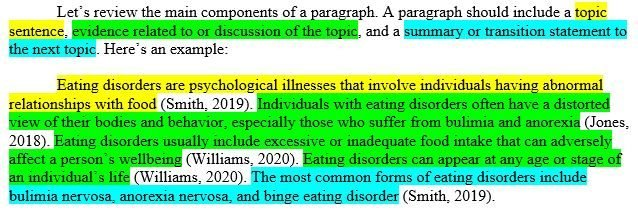
\includegraphics{cover.jpg}}
\begin{document}
\frame{\titlepage}

\floatname{algorithm}{Algorithm}


\begin{frame}{Slide}
\phantomsection\label{slide}
\begin{alertblock}{Alert block}
\phantomsection\label{alert-block}
Content
\end{alertblock}

\begin{exampleblock}{Example block}
\phantomsection\label{example-block}
Content

\begin{itemize}[<+->]
\tightlist
\item
  Eat spaghetti
\item
  Drink wine
\end{itemize}
\end{exampleblock}
\end{frame}

\begin{frame}{Slide with a pause}
\phantomsection\label{slide-with-a-pause}
content before the pause

\pause

content after the pause
\end{frame}

\begin{frame}{Multiple Columns}
\phantomsection\label{multiple-columns}
\begin{columns}[T]
\begin{column}{0.4\linewidth}
contents\ldots{}
\end{column}

\begin{column}{0.6\linewidth}
contents\ldots{}
\end{column}
\end{columns}

\begin{exampleblock}{Example block}
\phantomsection\label{example-block-1}
Content
\end{exampleblock}
\end{frame}

\begin{frame}{There Is No Largest Prime Number}
\phantomsection\label{there-is-no-largest-prime-number}
\framesubtitle{The proof uses \textit{reductio ad absurdum}.}
\begin{theorem}
There is no largest prime number.
\end{theorem}
\begin{proof}
\begin{enumerate}
\item<1-| alert@1> Suppose $p$ were the largest prime number.
\item<2-> Let $q$ be the product of the first $p$ numbers.
\item<3-> Then $q+1$ is not divisible by any of them.
\item<1-> Thus $q+1$ is also prime and greater than $p$.\qedhere
\end{enumerate}
\end{proof}
\end{frame}

\begin{frame}{There Is No Largest Prime Number}
\phantomsection\label{there-is-no-largest-prime-number-1}
\framesubtitle{The proof uses \textit{reductio ad absurdum}.}
\begin{theorem}
There is no largest prime number.
\end{theorem}
\begin{proof}

1. Suppose $p$ were the largest prime number.
2. Let $q$ be the product of the first $p$ numbers.
3. Then $q+1$ is not divisible by any of them.
4. Thus $q+1$ is also prime and greater than $p$.\qedhere

\end{proof}
\end{frame}

\begin{frame}{Training Deep Neural Networks}
\phantomsection\label{training-deep-neural-networks}
\begin{tikzpicture}[remember picture, overlay]
\node[anchor=north west, inner sep=0] at ([xshift=20pt, yshift=-20pt]current page.north west) {\includegraphics[width=40pt]{logo.png}};
    \node[anchor=north east, inner sep=0] at ([xshift=-20pt, yshift=-20pt]current page.north east) {\includegraphics[width=100pt]{youtube.png}};
    \draw[accentcolor, line width=2pt] ([yshift=-20pt]current page.north west) -- ([yshift=-20pt]current page.north east);
\end{tikzpicture}

\vspace{10pt}

\% Add vertical spacing

\begin{flushleft}
    \textbf{Maziar Raissi}

    Assistant Professor \\
    Department of Applied Mathematics \\
    University of Colorado Boulder \\
    \texttt{maziar.raissi@colorado.edu}
\end{flushleft}
\end{frame}




\end{document}
